% Results Part Three: Validation of CNN predictions

\subsection{Validation of CNN predictions}

% Figure 4: Validation of CNN Predictions
\begin{figure}[htbp]
    \centering
    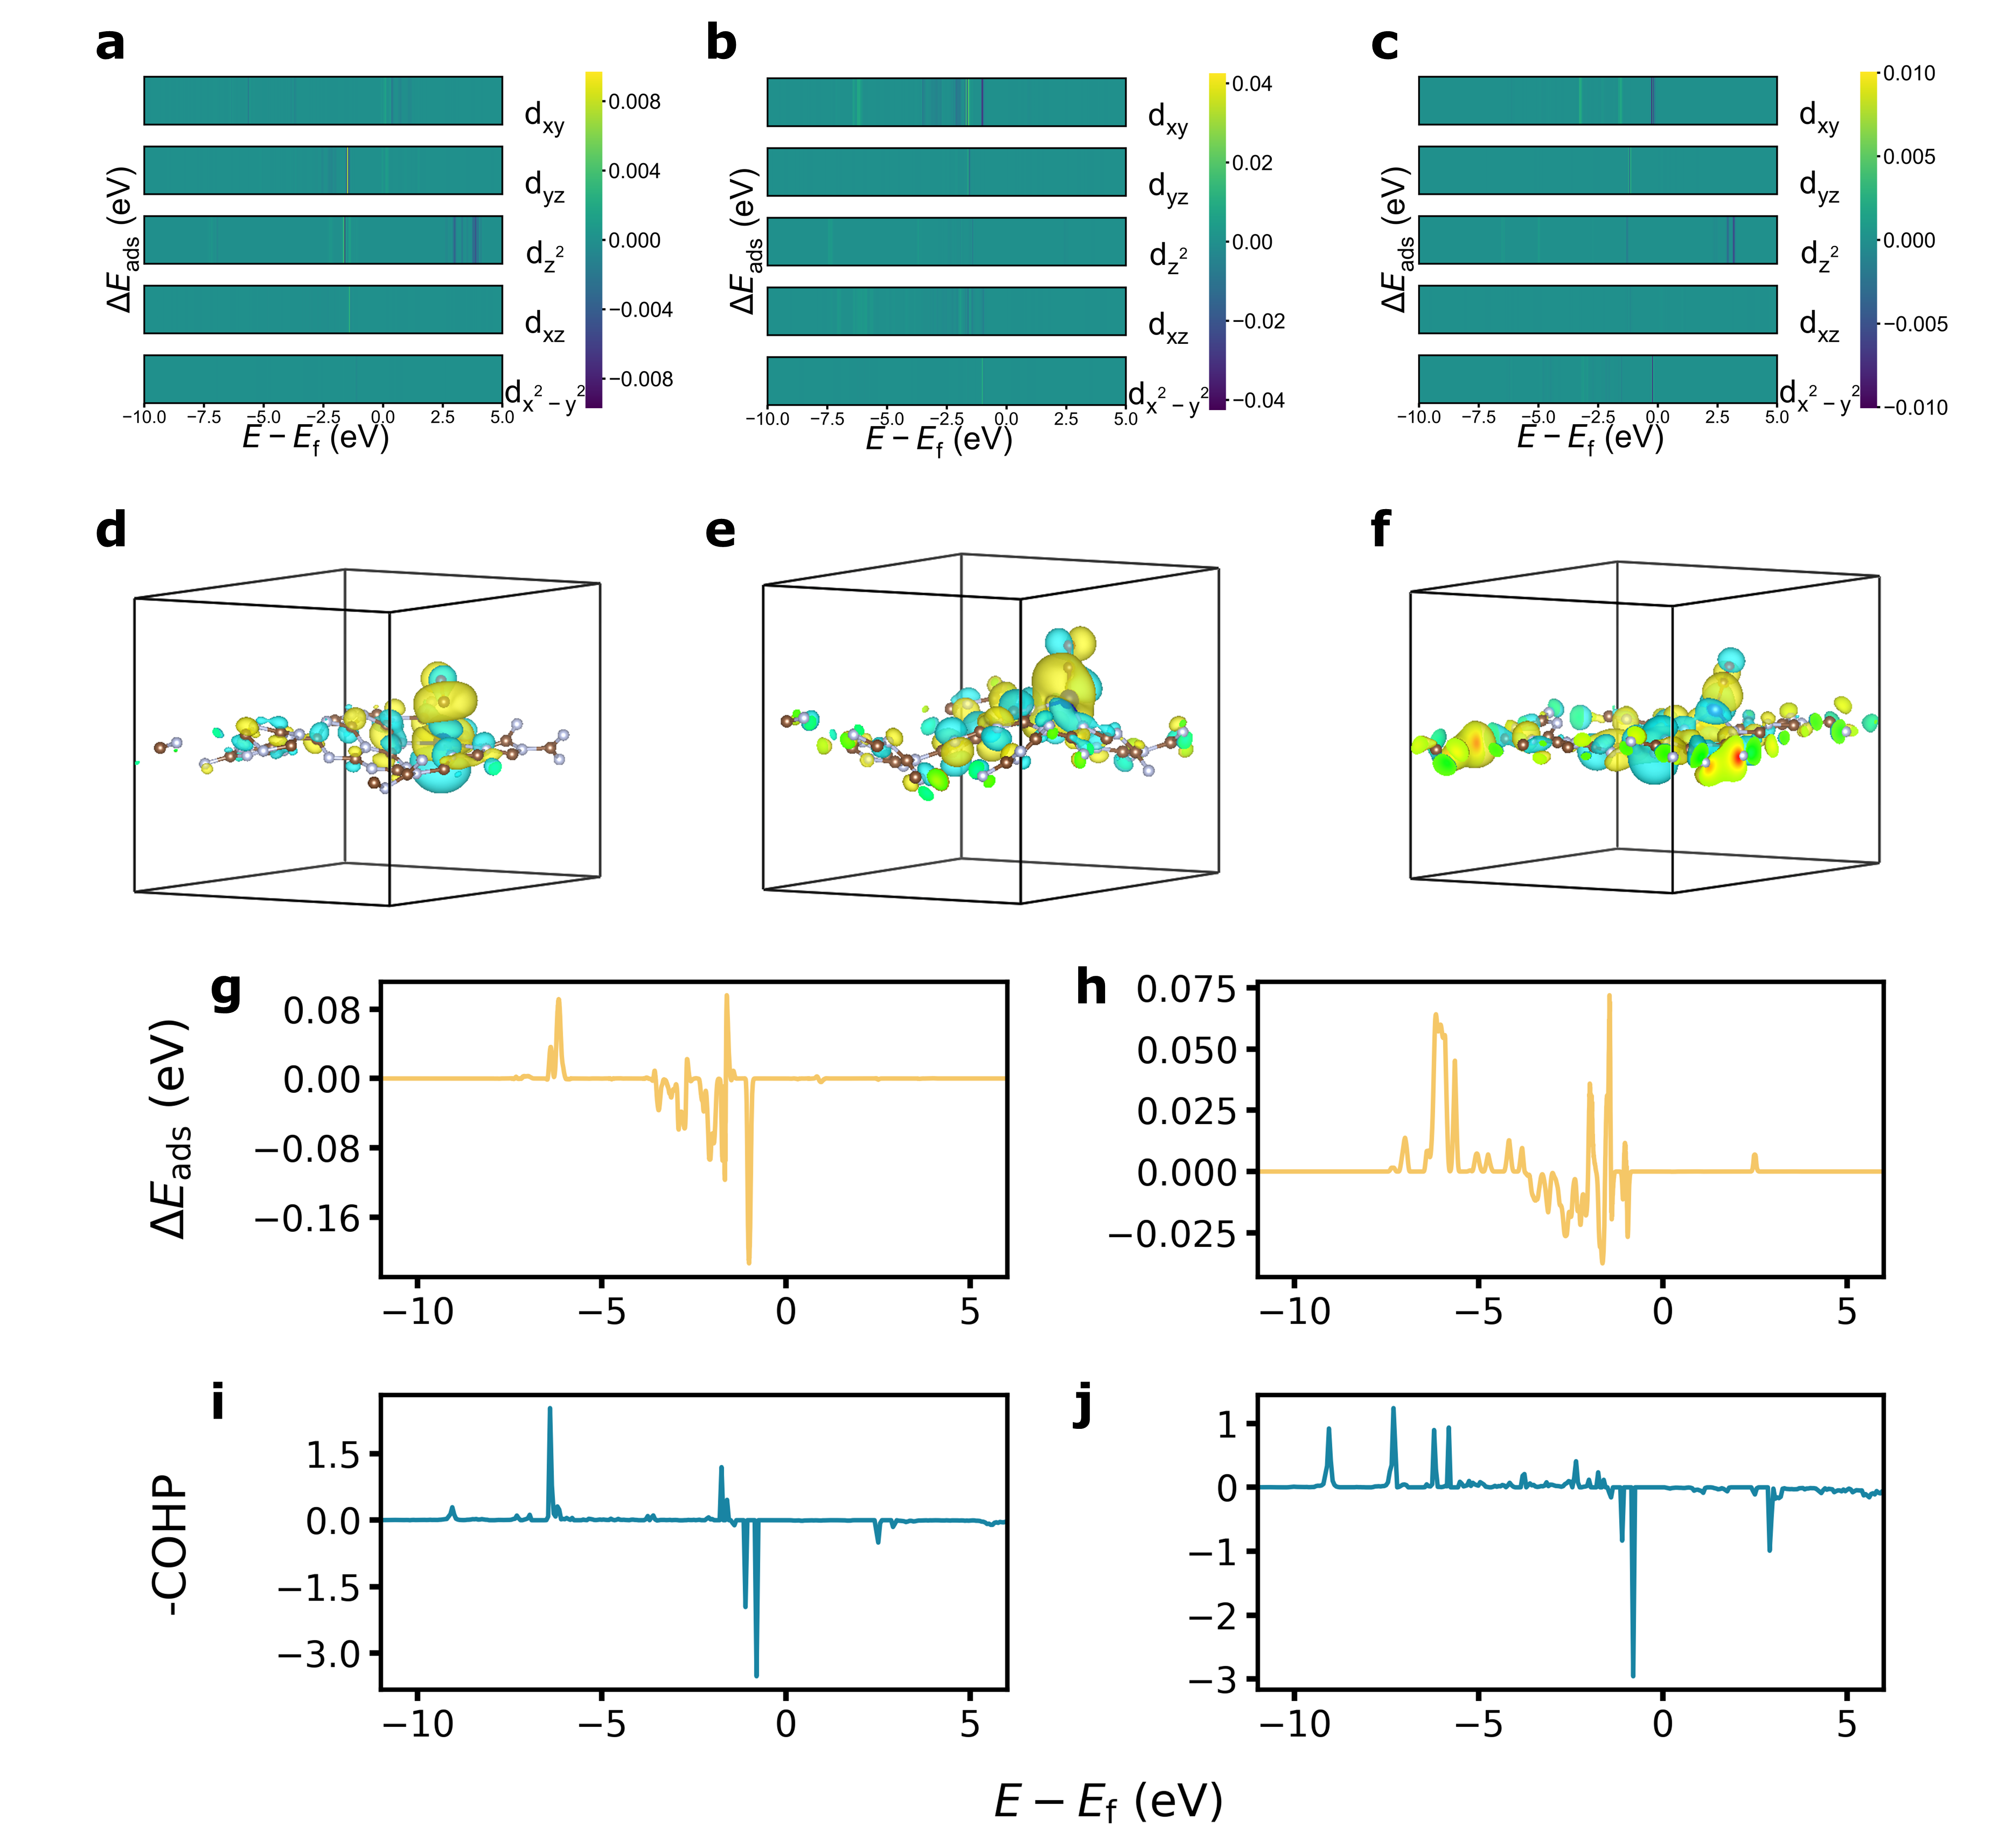
\includegraphics[width=\textwidth]{main_fig4_validation.png}
    \caption{\textbf{Validation of CNN predictions.}
    \textbf{a}-\textbf{c}, The eDOS occlusion experiment results for
    (\textbf{a}) Cr of Cr@g-C\textsubscript{3}N\textsubscript{4},
    (\textbf{b}) Co of Co@g-C\textsubscript{3}N\textsubscript{4} and
    (\textbf{c}) Cu of Cu@g-C\textsubscript{3}N\textsubscript{4}.
    eDOS occlusion experiments were conducted on the initial states of CO adsorption process.
    \textbf{d}-\textbf{f}, Real-space wavefunction visualization for
    (\textbf{d}) Cr $d_{x^2-y^2}$ orbital of Cr@g-C\textsubscript{3}N\textsubscript{4},
    (\textbf{e}) Co $d_{xy}$ orbital of Co@g-C\textsubscript{3}N\textsubscript{4} and
    (\textbf{f}) Cu $d_{xy}$ orbital of Cu@g-C\textsubscript{3}N\textsubscript{4}.
    Wavefunction visualizations were performed on the final states of CO adsorption process.
    The yellow and aqua colors represent areas of positive and negative
    Kohn-Sham orbital coefficients, respectively.
    \textbf{g}-\textbf{j}, Occlusion experiment results for (\textbf{g}) $d_{xy}$ orbital
    and (\textbf{h}) $d_{xz}$ orbital for Co of Co@g-C\textsubscript{3}N\textsubscript{4}.
    COHP analysis for (\textbf{i}) $d_{xy}$ orbital and (\textbf{j}) $d_{xz}$ orbital for
    Co of Co@g-C\textsubscript{3}N\textsubscript{4}, performed between Co and
    all adsorbate atoms in the final states of CO adsorption process.}
    \label{main_fig4:validation}
\end{figure}

Historically, interpretability has posed challenges for deep learning methods, often rendering their inner workings akin to black boxes \cite{zhang2018interpretable, zhang2018visual, savage2022breaking}.
The occlusion technique, widely utilized in Computer Vision \cite{zeiler2014visualizing, kortylewski2020combining, wang2020robust}, involves systematically masking sections of the input matrix to assess their impact on the final prediction score.
In our work, we introduce an orbitalwise occlusion method to discern individual orbital contribution to adsorption energy within the CNN model, drawing inspiration from Fung's pioneer integration of this technique into eDOS analysis \cite{fung2021machine}.
In this work, occlusion experiments involve orbitalwise masking specific eDOS, which are then fed into the CNN model to observe resulting disturbance in adsorption energy.
A visual representation of this process can be found in Supplementary \cref{supp_fig21:occlusion}. Conceptually, this experiment simulates the effect of shielding electronic states, allowing investigation of the potential contribution to adsorption energy from these states.
Additionally, we attempted to extract the planewave coefficients of Kohn-Sham orbital for wavefunction visualization.
This validation step was undertaken to confirm the spatial distribution of the orbitals pinpointed by the occlusion experiments.

To validate our method, we conducted occlusion experiments on Cr@g-C\textsubscript{3}N\textsubscript{4}, Co@g-C\textsubscript{3}N\textsubscript{4} and Cu@g-C\textsubscript{3}N\textsubscript{4}.
Each of these supported metals possesses 3d subshells with different electronic configurations: half-filled, partially filled and fully filled, allowing us to test the universality of our approach.
The results of the occlusion experiment on the supported Cr single atom in Cr@g-C\textsubscript{3}N\textsubscript{4} are given in \cref{main_fig4:validation}a.
The $d_{x^2-y^2}$ orbital emerges as dominant in CO interaction.
Shielding electrons centered around -2 eV significantly alter the adsorption energy, indicating the potency of this orbital.
The real-space wavefunction visualization in \cref{main_fig4:validation}d corroborates these findings, highlighting the interaction between the $d_{x^2-y^2}$ orbital of single metal atom and the adsorbate.
This suggests the $d_{x^2-y^2}$ orbital of supported Co predominantly influence the interaction with CO, and thus shielding electrons from this orbital markedly disturb the adsorption energy.
Additionally, occlusion experiments were performed on the Co $d_xy$ orbital of Co@g-C\textsubscript{3}N\textsubscript{4} (\cref{main_fig4:validation}b) and the $Cu d_xy$ orbital of Cu@g-C\textsubscript{3}N\textsubscript{4} (\cref{main_fig4:validation}c).
In both cases, the $d_xy$ orbital was identified as the dominant contributor.
While identifying the dominant orbital is crucial, these findings also suggest that interactions with adsorbates occurring out-of-plane are influenced by in-plane orbitals as well.
Importantly, it becomes evident that d orbitals do not universally impact interactions with adsorbates, emphasizing the need for case-specific discussions.

To validate the chemical relevance of predictions made by CNN model, we conducted COHP analysis, a theoretical bond-detecting tool used to identify bonding and anti-bonding contributions to band-structure energy \cite{deringer2011crystal}.
In this research, interactions between the supported metal atom and atoms within a 5 \text{\AA} radius were calculated to understand its bonding environment, as detailed in the Methods section.
The results of the occlusion experiment on the Co $d_xy$ orbital of Co@g-C\textsubscript{3}N\textsubscript{4}, identified as the dominant orbital via occlusion experiments, were compared with the COHP analysis, as shown in \cref{main_fig4:validation}g and \cref{main_fig4:validation}i.
The occlusion experiment pinpointed strong metal-adsorbate interactions at energy levels of -1 eV and -6.3 eV, which were confirmed by the COHP analysis.
We then investigated the non-dominant Co $d_xz$ orbital, and the COHP analysis highlighted interactions at -1 eV and -6.5 eV, aligning with the findings from the occlusion experiments.

In summary, orbitalwise occlusion experiments provide chemical interpretations into deep learning models, enhancing their interpretability.
Furthermore, these occlusion results are readily understandable to chemists, enabling the identification of orbitalwise contributions to the adsorption process.
